         \chapter{Electric circuits}\fancyfoot[LO,RE]{Focus Area: Physics}

    \setcounter{figure}{1}
    \setcounter{subfigure}{1}
    \label{f13bac5321b85aca0e213ebdf4f72465}
         \section{ Introduction and key concepts}
    \nopagebreak
            \label{m38771} $ \hspace{-5pt}\begin{array}{cccccccccccc}   
\includegraphics[width=0.75cm]{col11305.imgs/summary_fullmarks.png} &   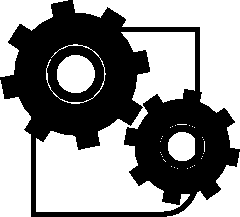
\includegraphics[width=0.75cm]{col11305.imgs/summary_simulation.png} &   \end{array} $ \hspace{2 pt}\raisebox{-5 pt}{} {(section shortcode: P10074 )} \par 
    \label{m38771*cid2}
            \subsection{ Electric Circuits}
            \nopagebreak
      \label{m38771*id62184}People all over the world depend on electricity to provide power for most appliances in the home and at work. For example, fluorescent lights, electric heating and cooking (on electric stoves), all depend on electricity to work.
To realise just how big an impact electricity has on our daily lives, just think about what happens when there is a power
failure or load shedding.\par 
\label{m38771*secfhsst!!!underscore!!!id72}
            \begin{groupdiscussion}{Uses of electricity }
            \nopagebreak
      \label{m38771*id62198}With a partner, take the following topics and, for each topic, write down at least 5 items/appliances/machines which need
electricity to work. Try not to use the same item more than once.\par 
      \label{m38771*id62544}\begin{itemize}[noitemsep]
            \label{m38771*uid1}\item At home
\label{m38771*uid2}\item At school
\label{m38771*uid3}\item At the hospital
\label{m38771*uid4}\item In the city
\end{itemize}
      \label{m38771*id62592}Once you have finished making your lists, compare with the lists of other people in your class. (Save your lists somewhere safe for later because there will be another activity for which you'll need them.)\par 
      \label{m38771*id62597}When you start comparing, you should notice that there are many different items which we use in our daily lives which rely on electricity to work!
      \end{groupdiscussion}
 \par 
\label{m38771*notfhsst!!!underscore!!!id89}
\begin{tabular}{cc}
	   \hspace*{-50pt}\raisebox{-8 mm}{ 
\includegraphics[width=0.5in]{col11305.imgs/pstip2.png}  }& 
	\Tip{\textbf{Safety Warning:}
We believe in experimenting and learning about physics at every opportunity, BUT
playing with electricity and electrical appliances can be \textbf{EXTREMELY DANGEROUS}! Do not try to build
homemade circuits alone. Make sure you have someone with you who knows if what you are doing is safe.
Normal electrical outlets are dangerous. Treat electricity with respect in your everyday life. Do not touch exposed wires and do not approach downed power lines.}
	\end{tabular}
	\par
      \label{m38771*uid5}
            \subsubsection{ Closed circuits}
            \nopagebreak
        \label{m38771*id62637}In the following activity we will investigate what is needed to cause charge to flow in an electric circuit.\par 
\label{m38771*secfhsst!!!underscore!!!id97}
            \begin{f_experiment}{Closed circuits}
            \nopagebreak
            \label{m38771*id62648}\noindent{}\textbf{Aim:}
To determine what is required to make electrical charges flow.
In this experiment, we will use a lightbulb to check whether electrical charge is flowing in the circuit or not. If charge is flowing, the lightbulb should glow. On the other hand, if no charge is flowing, the lightbulb will not glow.\par 
        \label{m38771*id62665}\noindent{}\textbf{Apparatus:}
        You will need a small lightbulb which is attached to a metal conductor (e.g. a bulb from a school electrical kit), some connecting wires and a battery.\par 
        \label{m38771*id62679}\noindent{}\textbf{Method:}
        Take the apparatus items and try to connect them in a way that you cause the light bulb to glow (i.e. charge flows in the circuit).\par 
        \label{m38771*id62694}\noindent{}\textbf{Questions:}
        \label{m38771*id62702}\begin{enumerate}[noitemsep, label=\textbf{\arabic*}. ] 
            \label{m38771*uid6}\item Once you have arranged your circuit elements to make the lightbulb glow, draw your circuit.
\label{m38771*uid7}\item What can you say about how the battery is connected? (i.e. does it have one or two connecting leads attached? Where are they attached?)
\label{m38771*uid8}\item What can you say about how the light bulb is connected in your circuit? (i.e. does it connect to one or two connecting leads, and where are they attached?)
\label{m38771*uid9}\item Are there any items in your circuit which are not attached to something? In other words, are there any gaps in your circuit?
\end{enumerate}
        \par 
        \label{m38771*id62757}Write down your conclusion about what is needed to make an electric circuit work and charge to flow.
 \par\end{f_experiment}

        \label{m38771*id62768}In the experiment above, you will have seen that the light bulb only glows when there is a \textsl{closed} circuit i.e. there are no gaps in the circuit and all the circuit elements are connected in a \textsl{closed loop}. Therefore, in order for charges to flow, a closed circuit and an energy source (in this case the battery) are needed. (Note: you do not have to have a lightbulb in the circuit! We used this as a check that charge was flowing.)\par 
\label{m38771*fhsst!!!underscore!!!id128}
\Definition{   \label{id2477990}\textbf{ Electric circuit }} { \label{m38771*meaningfhsst!!!underscore!!!id128}
        \label{m38771*id62792}An electric circuit is a closed path (with no breaks or gaps) along which electrical charges (electrons) flow powered by an energy source. \par 
         } 
         \Warning{Don't use your body to complete the circuit!}
   
      \label{m38771*uid10}
            \subsubsection{ Representing electric circuits}
            \nopagebreak
        \label{m38771*uid11}
            \subsubsection{ Components of electrical circuits}
            \nopagebreak
          \label{m38771*id62821}Some common elements (components) which can be found in electrical circuits include light bulbs, batteries, connecting leads, switches, resistors, voltmeters and ammeters. You will learn more about these items in later sections, but it is important to know what their symbols are and how to represent them in circuit diagrams. Below is a table with the items and their symbols:\par 
    % \textbf{m38516*uid12}\par
          \begin{table}[H]
    % \begin{table}[H]
    % \\ '' '0'
        \begin{center}
      \label{m38773*id67892}
    \noindent
    \tabletail{%
        \hline
        \multicolumn{3}{|p{\mytableboxwidth}|}{\raggedleft \small \sl continued on next page}\\
        \hline
      }
      \tablelasttail{}
      \begin{xtabular}[t]{|l|l|l|}\hline
                  \textbf{Instrument}
                 &
                  \textbf{Measured Quantity}
                 &
                  \textbf{Proper Connection}
                % make-rowspan-placeholders
     \tabularnewline\cline{1-1}\cline{2-2}\cline{3-3}
      %--------------------------------------------------------------------
        Voltmeter &
        Voltage &
        In Parallel% make-rowspan-placeholders
     \tabularnewline\cline{1-1}\cline{2-2}\cline{3-3}
      %--------------------------------------------------------------------
        Ammeter &
        Current &
        In Series% make-rowspan-placeholders
     \tabularnewline\cline{1-1}\cline{2-2}\cline{3-3}
      %--------------------------------------------------------------------
    \end{xtabular}
      \end{center}
    \begin{center}{\small\bfseries Table 16.2}\end{center}
    \begin{caption}{\small\bfseries Table 16.2}\end{caption}
\end{table}
    \par
  \label{m38773**end}
  \chapter{Resistance is Futile}%\fancyfoot[LO,RE]{Focus Area: Chemistry}
  
         \section{ Resistance}
    \nopagebreak
            \label{m38776} $ \hspace{-5pt}\begin{array}{cccccccccccc}   
\includegraphics[width=0.75cm]{col11305.imgs/summary_fullmarks.png} &   
\includegraphics[width=0.75cm]{col11305.imgs/summary_video.png} &   \end{array} $ \hspace{2 pt}\raisebox{-5 pt}{} {(section shortcode: P10077 )} \par 
    \label{m38776*cid5}
            \subsection{ Resistance}
            \nopagebreak
      \label{m38776*sb1235}
	The resistance of a circuit element can be thought of as how much it opposes the flow of electric current in the circuit. 
	\vspace{\rubberspace}\par
	\Definition{   \label{id2485077}\textbf{ Resistance }} { \label{m38776*meaningfhsst!!!underscore!!!id1729}
        \label{m38776*id67260} The resistance of a conductor is defined as the potential difference across it divided by the current flowing though it. We use the symbol \textbf{R} to show resistance and it is measured in units called \textbf{Ohms} with the symbol $\mathrm{\Omega }$.\par 
        \label{m38776*id67288}\nopagebreak\noindent{}
          
    \begin{equation}
    1\phantom{\rule{4pt}{0ex}}\mathrm{Ohm}=1\frac{\mathrm{Volt}}{\mathrm{Ampere}}.\tag{16.30}
      \end{equation}
         } 
      \end{tabular*}
	\par 
      \label{m38776*uid62}
            \subsubsection{ What causes resistance?}
            \nopagebreak
        \label{m38776*id67246}We have spoken about resistors that reduce the flow of charge
in a conductor. On a microscopic level, electrons moving through
the conductor collide with the particles of which the conductor
(metal) is made. When they collide, they transfer kinetic energy.
The electrons lose kinetic energy and slow down. This leads to
resistance. The transferred energy causes the resistor to heat up.
You can feel this directly if you touch a cellphone charger when you are charging a cell phone - the charger gets warm because its circuits have some resistors in them!\par 
        \label{m38776*id67330}\textsl{All} conductors have some resistance. For example, a piece of wire
has less resistance than a light bulb, but both have resistance. A lightbulb is a very thin wire surrounded by a glass housing The high resistance of the filament (small wire) in a lightbulb causes the electrons to
transfer a lot of their kinetic energy in the form of heat\label{m38776*uid63}\footnote{Flourescent lightbulbs do not use thin wires; they use the fact that certain gases glow when a current flows through them. They are much more efficient (much less resistance) than lightbulbs.}. The heat energy is enough
to cause the filament to glow white-hot which produces light. The wires
connecting the lamp to the cell or battery hardly even get warm while
conducting the same amount of current. This is because of their
much lower resistance due to their larger cross-section (they are thicker).\par 
        \label{m38776*id67354}An important effect of a resistor is that it \textsl{converts} electrical
energy into \textbf{heat} energy. \textbf{Light} is a by-product of the heat that is produced.\par 
\label{m38776*notfhsst!!!underscore!!!id1758}
\begin{tabular}{cc}
	\hspace*{-50pt}\raisebox{-8 mm}{\hspace{-0.2in}
\includegraphics[width=0.75in]{col11305.imgs/psfact2.png} } & 
	\Tip{There is a special type of conductor,
called a \textbf{superconductor} that has no resistance, but the
materials that make up all known superconductors only start superconducting
at very low temperatures (approximately -170${}^{\circ }$C).}
	\end{tabular}
	\par
 \label{m38776*uid64}
            \begin{activity}{ Why do batteries go flat?}
            \nopagebreak
            \begin{minipage}{.5\columnwidth}
          \label{m38776*id67413}A battery stores chemical potential energy. When it is connected in a circuit, a chemical reaction takes place inside the battery which converts chemical potential energy to electrical energy which powers the charges (electrons) to move through the circuit. All the circuit elements (such as the conducting leads, resistors and lightbulbs) have some resistance to the flow of charge and convert the electrical energy to heat and, in the case of the lightbulb, heat and light.
Since energy is always conserved, the battery goes flat when all its chemical potential energy has been converted into other forms of energy.\par 
      \label{m38776*uid65}\end{minipage}
            \begin{minipage}{.5\columnwidth}
	\includegraphics[width=0.75in]{photos/batterystack.jpg} } 
            \end{minipage}
      \end{activity}
            \subsubsection{ Resistors in electric circuits}
            \nopagebreak
        \label{m38776*id67431}It is important to understand what effect adding resistors to a circuit has on the \textsl{total} resistance of a circuit and on the current that can flow in the circuit.\par 
        \label{m38776*uid66}
            \subsubsection{ Resistors in series}
            \nopagebreak
          \label{m38776*id67450}When we add resistors in series to a circuit, we \textsl{increase} the resistance to the flow of current. There is only \textbf{one path} along which the current can flow and the current is the same at all places in the series circuit. Take a look at the diagram below: On the left there is a circuit with a single resistor and a battery. No matter where we measure the current, it is the same in a series circuit. On the right, we have added a second resistor in series to the circuit. The \textsl{total} resistance of the circuit has \textsl{increased} and you can see from the reading on the ammeter that the current in the circuit has \textsl{decreased} and is still the same everywhere in the circuit.\par 
          \label{m38776*id67481}
    \setcounter{subfigure}{0}
	\begin{figure}[H] % horizontal\label{m38776*id67485}
    \begin{center}
    \label{m38776*id67485!!!underscore!!!media}\label{m38776*id67485!!!underscore!!!printimage}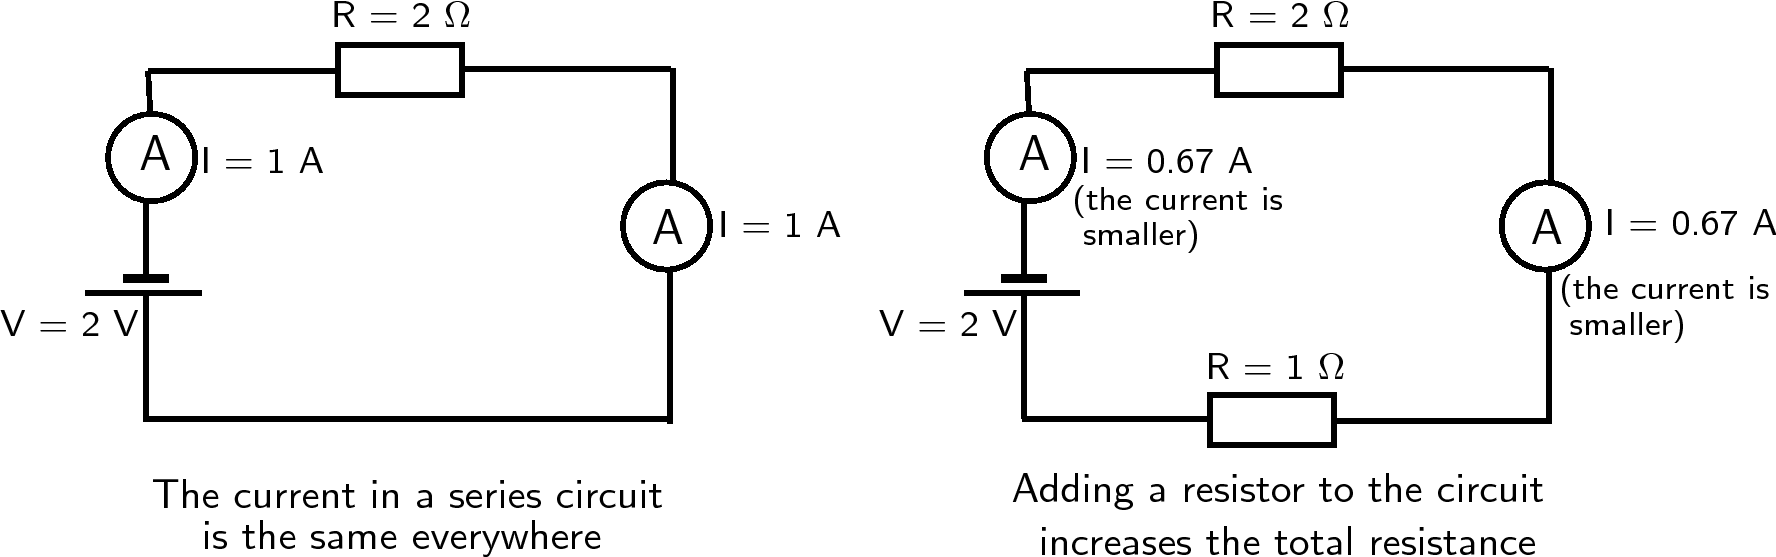
\includegraphics{col11305.imgs/m38776_PG10C9_032.png} % m38776;PG10C9\_032.png;;;6.0;8.5;
      \vspace{2pt}
    \vspace{.1in}
    \end{center}
 \end{figure}       
          \par 
            \subsubsection{ Equivalent Series Resistance}
            \nopagebreak
            \label{m38776*id63926}When there is more than one resistor in a circuit, we are usually able to calculate the total combined resitance of all the resistors. The resistance of the single resistor is known as \textsl{equivalent resistance} or total resistance.
Consider a circuit consisting of three resistors and a single cell connected in series.\par 
          \label{m38776*id63930}
    \setcounter{subfigure}{0}
	\begin{figure}[H] % horizontal\label{m38776*id63934}
    \begin{center}
    \label{m38776*id63934!!!underscore!!!media}\label{m38776*id63934!!!underscore!!!printimage}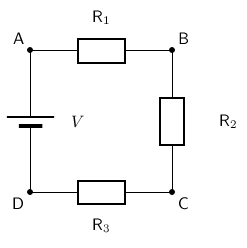
\includegraphics[width=0.4\columnwidth]{col11305.imgs/m38776_PG11C9_007.png} % m38776;PG11C9\_007.png;;;6.0;8.5;
      \vspace{2pt}
    \vspace{.1in}
    \end{center}
 \end{figure}       
          \par 
\label{m38776*eip-546}We can define the total resistance in a series circuit as:\par \label{m38776*fhsst!!!underscore!!!id788}
	\Definition{   \label{id2485652}\textbf{ Equivalent resistance in a series circuit, ${R}_{s}$ }} { \label{m38776*meaningfhsst!!!underscore!!!id788}
          \label{m38776*id64628}For $n$ resistors in series the equivalent resistance is:\par 
          \label{m38776*uid2532}\nopagebreak\noindent{}
            
    \begin{equation}
    {R}_{s}={R}_{1}+{R}_{2}+{R}_{3}+\cdots +{R}_{n}\tag{16.31}
      \end{equation}
           } 
          \label{m38776*id64719}The more resistors we add in series, the higher the equivalent resistance in the circuit. Since the resistors act as obstacles to the flow of charge through the circuit, the current in the circuit is reduced. Therefore, the \textsl{higher} the resistance in the circuit, the \textsl{lower} the current through the battery and the circuit. We say that the current in the battery is inversely proportional to the resistance in the circuit. 
Let us apply the rule of equivalent resistance in a series circuit to the following circuit.\par 
          \label{m38776*id64722}
    \setcounter{subfigure}{0}
	\begin{figure}[H] % horizontal\label{m38776*id64726}
    \begin{center}
    \label{m38776*id64726!!!underscore!!!media}\label{m38776*id64726!!!underscore!!!printimage}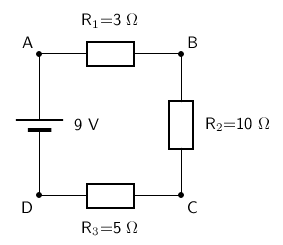
\includegraphics[width=0.4\columnwidth]{col11305.imgs/m38776_PG11C9_008.png} % m38776;PG11C9\_008.png;;;6.0;8.5;
      \vspace{2pt}
    \vspace{.1in}
    \end{center}
 \end{figure}       
          \par 
          \label{m38776*id64732}The resistors are in series, therefore:\par 
          \label{m38776*id64736}\nopagebreak\noindent{}
    \begin{equation}
    \begin{array}{ccc}\hfill {R}_{s}& =& {R}_{1}+{R}_{2}+{R}_{3}\hfill \\ & =& 3\phantom{\rule{0.166667em}{0ex}}\mathrm{\Omega }+10\phantom{\rule{0.166667em}{0ex}}\mathrm{\Omega }+5\phantom{\rule{0.166667em}{0ex}}\mathrm{\Omega }\hfill \\ & =& 18\phantom{\rule{0.166667em}{0ex}}\mathrm{\Omega }\hfill \end{array}\tag{16.32}
      \end{equation}
\label{m38776*eip-186}
            \begin{i_experiment}{Current in Series Circuits}
            \nopagebreak
            \label{m38776*id66871}\noindent{}\textbf{Aim:}
          To determine the effect of multiple resistors on current in a circuit\par 
        \label{m38776*id66886}\noindent{}\textbf{Apparatus:}
        \label{m38776*id66895}\begin{itemize}[noitemsep]
            \label{m38776*uid49}\item Battery
\label{m38776*uid50}\item Resistors
\label{m38776*uid51}\item Light bulb
\label{m38776*uid52}\item Wires
\end{itemize}
        \par 
        \label{m38776*id66948}\noindent{}\textbf{Method:}
        \label{m38776*id66957}\begin{enumerate}[noitemsep, label=\textbf{\arabic*}. ] 
            \label{m38776*uid53}\item Construct the following circuits
    \setcounter{subfigure}{0}
	\begin{figure}[H] % horizontal\label{m38776*id66976}
    \begin{center}
    \label{m38776*id66976!!!underscore!!!media}\label{m38776*id66976!!!underscore!!!printimage}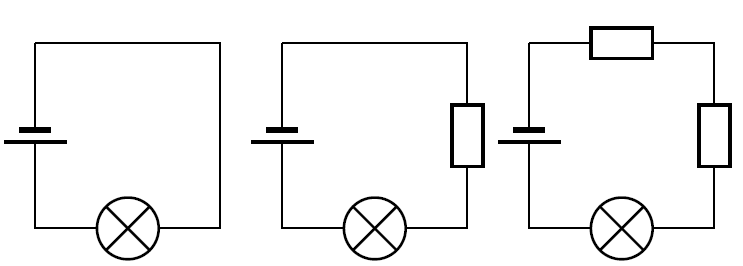
\includegraphics[width=\columnwidth]{col11305.imgs/m38776_PG10C9_027.png} % m38776;PG10C9\_027.png;;;6.0;8.5;
      \vspace{2pt}
    \vspace{.1in}
    \end{center}
 \end{figure}       \label{m38776*uid54}\item Rank the three circuits in terms of the brightness of the bulb.
\end{enumerate}
        \par 
        \label{m38776*id66996}\noindent{}\textbf{Conclusions:}
        The brightness of the bulb is an indicator of how much current is flowing. If the bulb gets brighter because of a change then more current is flowing. If the bulb gets dimmer less current is flowing.
You will find that the more resistors you have the dimmer the bulb.
 \par 
 \end{i_experiment}
\label{m38776*secfhsst!!!underscore!!!id903}\vspace{.5cm} 
      \noindent
      \begin{wex}{Equivalent series resistance I}{
          \label{m38776*probfhsst!!!underscore!!!id904}
          \label{m38776*id64862}Two 10 k$\Omega $ resistors are connected in series. Calculate the equivalent resistance. \par 
          \vspace{5pt}}{
          \label{m38776*solfhsst!!!underscore!!!id907}\noindent\textbf{Solution to Exercise } \label{m38776*listfhsst!!!underscore!!!id907}\begin{enumerate}[noitemsep, label=\textbf{Step} \textbf{\arabic*}. ] 
            \leftskip=20pt\rightskip=\leftskip\item  
          \label{m38776*id64896}Since the resistors are in series we can use:\par 
          \label{m38776*id64899}\nopagebreak\noindent{}
            
    \begin{equation}
    {R}_{s}={R}_{1}+{R}_{2}\tag{16.33}
      \end{equation}
          \item  
          \label{m38776*id64940}\nopagebreak\noindent{}
            
    \begin{equation}
    \begin{array}{ccc}\hfill {R}_{s}& =& {R}_{1}+{R}_{2}\hfill \\ & =& 10\phantom{\rule{0.166667em}{0ex}}\mathrm{k}\phantom{\rule{0.166667em}{0ex}}\Omega +10\phantom{\rule{0.166667em}{0ex}}\mathrm{k}\phantom{\rule{0.166667em}{0ex}}\Omega \hfill \\ & =& 20\phantom{\rule{0.166667em}{0ex}}\mathrm{k}\phantom{\rule{0.166667em}{0ex}}\Omega \hfill \end{array}\tag{16.34}
      \end{equation}
          \item  
          \label{m38776*id65061}The equivalent resistance of two 10 k$\Omega $ resistors connected in series is 20 k$\Omega $. \par 
          \end{enumerate}}
    \end{wex}
    \noindent
\label{m38776*secfhsst!!!underscore!!!id1001}\vspace{.5cm} 
      \noindent
      \hspace*{-30pt}
\includegraphics[width=0.5in]{col11305.imgs/pspencil2.png}   \raisebox{25mm}{   
      \begin{wex}{Equivalent series resistance II }{
          \label{m38776*probfhsst!!!underscore!!!id1002}
          \label{m38776*id65108}Two resistors are connected in series. The equivalent resistance is 100 $\Omega $. If one resistor is 10 $\Omega $, calculate the value of the second resistor. \par 
          \vspace{5pt}}{
          \label{m38776*solfhsst!!!underscore!!!id1005}\noindent\textbf{Solution to Exercise } \label{m38776*listfhsst!!!underscore!!!id1005}\begin{enumerate}[noitemsep, label=\textbf{Step} \textbf{\arabic*}. ] 
            \leftskip=20pt\rightskip=\leftskip\item  
          \label{m38776*id65152}Since the resistors are in series we can use:\par 
          \label{m38776*id65155}\nopagebreak\noindent{}
            
    \begin{equation}
    {R}_{s}={R}_{1}+{R}_{2}\tag{16.35}
      \end{equation}
          \label{m38776*id65192}We are given the value of ${R}_{s}$ and ${R}_{1}$.\par 
          \item  
          \label{m38776*id65230}\nopagebreak\noindent{}
            
    \begin{equation}
    \begin{array}{ccc}\hfill {R}_{s}& =& {R}_{1}+{R}_{2}\hfill \\ \hfill \therefore {R}_{2}& =& {R}_{s}-{R}_{1}\hfill \\ & =& 100\phantom{\rule{0.166667em}{0ex}}\Omega -10\phantom{\rule{0.166667em}{0ex}}\Omega \hfill \\ & =& 90\phantom{\rule{0.166667em}{0ex}}\Omega \hfill \end{array}\tag{16.36}
      \end{equation}
          \item  
          \label{m38776*id65371}The second resistor has a resistance of 90 $\Omega $. \par 
          \end{enumerate}}
    \end{wex}
    }
    \noindent
    \setcounter{subfigure}{0}
